% Template for PLoS
% Version 1.0 January 2009
%
% To compile to pdf, run:
% latex plos.template
% bibtex plos.template
% latex plos.template
% latex plos.template
% dvipdf plos.template

\documentclass[10pt]{article}

% amsmath package, useful for mathematical formulas
\usepackage{amsmath}
% amssymb package, useful for mathematical symbols
\usepackage{amssymb}

% graphicx package, useful for including eps and pdf graphics
% include graphics with the command \includegraphics
\usepackage{graphicx}

% cite package, to clean up citations in the main text. Do not remove.
\usepackage{cite}

\usepackage{color} 

% Use doublespacing - comment out for single spacing
%\usepackage{setspace} 
%\doublespacing


% Text layout
\topmargin 0.0cm
\oddsidemargin 0.5cm
\evensidemargin 0.5cm
\textwidth 16cm 
\textheight 21cm

% Bold the 'Figure #' in the caption and separate it with a period
% Captions will be left justified
\usepackage[labelfont=bf,labelsep=period,justification=raggedright]{caption}

% Use the PLoS provided bibtex style
\bibliographystyle{plos2009}

% Remove brackets from numbering in List of References
\makeatletter
\renewcommand{\@biblabel}[1]{\quad#1.}
\makeatother


% Leave date blank
\date{}

\pagestyle{myheadings}
%% ** EDIT HERE **


%% ** EDIT HERE **
%% PLEASE INCLUDE ALL MACROS BELOW

%% END MACROS SECTION

\begin{document}

% Title must be 150 characters or less
\begin{flushleft}
{\Large
\textbf{A Federated Design for a Neurobiological Simulation Engine: The CBI framework for GENESIS 3.0}
}
% Insert Author names, affiliations and corresponding author email.
\\
Cornelis H.$^{1,\ast}$, 
Coop A. D.$^{2}$,
Bower J. M.$^{3}$.
\\
\bf{1} Cornelis H. Research Imaging Institute, University of Texas Health Science Center at San Antonio, San Antonio, TX, United States
\\
\bf{2} Coop A. D. Deptartment of Epidemiology and Biostatistics, University of Texas Health Science Center at San Antonio, San Antonio, TX, United States
\\
\bf{3} Bower J. M. Research Imaging Institute, University of Texas Health Science Center at San Antonio, San Antonio, TX, United States
\\
$\ast$ E-mail: Corresponding Hugo.Cornelis@gmail.com
\end{flushleft}

% Please keep the abstract between 250 and 300 words
\section*{Abstract}

The Computational Biology Initiative federated software architecture
was developed in response to a growing requirement in computational
biology for simulator interoperability and extensibility. It is
federated by its union of independent disparate systems under a single
cohesive view. It provides interoperability through its capability to
communicate, execute programs, or transfer data among different
independent applications. It supports extensibility through mechanisms
that enable simulator expansion or enhancement without the need for
major changes to system infrastructure.

Historically, simulator interoperability has relied on development of extensible markup languages such as the neuron modeling language NeuroML, while simulator extension typically occurred through modification of existing functionality.
The software architecture we describe allows for both these approaches. However, it is designed to support alternative paradigms of interoperability and extensibility through the provision of semantically defined application programming interfaces. They allow any appropriately configured component or software application to be incorporated into a simulator.

The architecture defines independent functional modules that run
stand-alone. They are arranged in logical layers that naturally
correspond to the occurrence of high-level data (biological concepts)
versus low-level data (numerical values) and distinguish data from
control functions.

Its modular nature and independence of technology facilitates communication about similar
concepts and functions between both users and developers.  It provides
important advantages for multiple independent contributions to
software development.  Importantly this includes: (1) Complexity of
individual simulator components is reduced compared to the complexity
of a complete simulator, (2) Components can be documented in
isolation, in terms of their inputs and outputs, (3) Unnecessary or
obsoleted components can easily be replaced or removed, (4) Components
can be tested stand-alone, and (5) The architecture clearly delineates
the development scope of new components.

Here, we review the recently reconfigured GENESIS 3.0 neural simulator and describe how it complies with the Computational Biology Initiative federated software architecture.

\marginpar{{\bf Hugo:} Currently 301 words, must be $\leq$\,300.}

%Software architectures can be described in different ways.  This paper
%describes the CBI simulator software architecture by putting
%stand-alone software components into a logically layered diagram.  The
%layers in the software architecture naturally correspond to the
%occurence of high-level data (e.g. biological concepts) versus
%low-level data (e.g.  numerical values).  This diagram can be used by
%users as well as developers to communicate about the global concepts
%and functions present in the software, independent of the used
%technology.
%
%Each software component is self-contained, in the sense that it can be
%run stand-alone. This has important advantages for
%facilitating contributions to software development from many people:
%
%\begin{itemize}
%\item The complexity of a single component is reduced compared to the
%  complexity of a complete software system.
%\item A component can be documented as an isolated entity, in terms of
%  inputs and outputs.  This facilitates the communication between
%  developers.
%\item When a component is considered not necessary or obsoleted, it
%  can be replaced, or removed from the architecture.
%\item From a developer perspective, a component can be tested
%  stand-alone.
%\item Most importantly, for new developments, the architecture clearly
%  delineates the scope of the development.  From the early start, new
%  components can be designed to fill only one component of the
%  architecture.
%\end{itemize}
%
%These properties facilitate the building and maintenance of a
%developer community, and the integration of new components.
%
%The CBI simulator software architecture is the result of a functional
%analysis of user requirements.  It indirectly represents the user
%needs, independent of concerns such as the technology used or the
%technical requirements (so also independent of the fact if it is
%technically possible to implement this architecture).  Since users can hook in
%extensions at a layer that is clearly defined, this analysis also
%provides an infrastructure for extensibility.
%
%discuss operations modelers perform on a model, taken from thesis
%
%say that a model evolves over time, discuss shortly the purkinje cell
%model, macro evolution.  Discuss operations in context of a data model
%?
%
%Relate the data model to an XML data model, more specifically neuroml data model.
%
%discuss the ndf data model, include an example.
%
%Link with
%http://en.wikipedia.org/wiki/High\_Level\_Architecture \\
%http://en.wikipedia.org/wiki/Levels\_of\_conceptual\_interoperability \\
%http://en.wikipedia.org/wiki/Data\_integration \\
%http://en.wikipedia.org/wiki/Abstraction\_layer \\
%
%accessibility for neuronal model parameters:
%
%e.g. conductance vs scaled conductance.
%
%conductance scaling contains a set of logic rules:
%1. for a simple compartment
%2. for a compartment with spines
%3. for specific membrane resistance.

\section*{Introduction}

The application of mathematical methods to modeling and quantification in neurophysiology can be traced to the Lapicque model of a neuron introduced over a century ago (Lapicque, 1907) the empirical description of action potential generation and propagation (Hodgkin \& Huxley, 1952), and the application of cable theory to the modeling of dendrites (Rall, 1957). Although, computer modeling was employed to verify the original integration of the action potential by a hand cranked calculator, it was not until the use of mathematical approaches based on cable theory were developed in the late 1950s to model dendritic properties and function (Rall, 1959), that digital computers became a necessary tool for modeling studies. It took a further quarter century for the interdisciplinary field that links neuroscience, cognitive science, electrical engineering, computer science, physics, and mathematics to be named and thus give birth to computational neuroscience (Schwartz, 1990).
%Since that time, a continued and rapid development of computer hardware and software has led to a plethora of systems for the description, simulation, and analysis of computational models from the sub-cellular (e.g. MCell--Stiles \& Bartoll, 2001; Roth et al., 2000) to large networks of biophysically realistic model neurons (e.g. Brunel \& Wang, 2001, Traub et al., 2005).

% Lapicque L (1907) Recherches quantitative sur l'excitabilitie electrique des nerfs traitee comme une polarisation. J Physiol Pathol Gen 9: 620--635.
% Hodgkin AL & Huxley AF (1952) A quantitative description of membrane current and its application to conduction and excitation in nerve. J Physiol 117: 500--544.
% Rall W (1957) Membrane time constants of motoneurons. Science 126:454.
% Rall W (1959) Branching dendritic trees and motoneuron membrane resistivity. Exp Neurol 1: 491--527.
% Schwartz E (1990). Computational Neuroscience. Cambridge, Mass: MIT Press
% Stiles JR \& Bartol TM (2001) Monte Carlo methods for simulating realistic synaptic microphysiology using MCell. In: E De Schutter (ed.) Computational Neuroscience: Realistic Modeling for Experimentalists. CRC Press: Boca Raton, pp. 87--127.
% Roth, A., Nusser, Z., & H�usser, M. (2000). Monte Carlo simulations of synaptic transmission in detailed three-dimensional reconstructions of cerebellar neuropil. Eur J Neurosci 12(Suppl. 11): 14.
% (2001). NEOSIM: Portable large-scale plug and play modelling. 
% Traub RD, Contreras D, Cunningham MO, Murray H, LeBeau FEN, Roopun A, Bibbig A, Wilent WB, Higley MJ \& Whittington MA (2005). Single-column thalamocortical network model exhibiting gamma oscillations, sleep spindles and  epileptogenic bursts. Journal of Neurophysiology 93: 2194--2232.
% Brunel N \& Wang X-J (2001) Effects of neuromodulation in a cortical network model of object working memory dominated by recurrent inhibition. J Comput Neurosci 11: 63--85.

Historically, the development of neuronal simulation software for the construction of morphologically detailed neuron models and small networks was instigated by research projects that specifically addressed complementary technical and scientific questions (Moore, 2010). For example, one widely used application is NEURON (Hines, 1993) which grew from the identification of numerical techniques that greatly improved both the efficient computation and accuracy of the solution to the cable equations used to model electrical activity in branched dendrites (Hines, 1984, 1988). Alternatively, another widely used simulation platform, GENESIS (Wilson et al., 1989,) was from its conception a more generalized simulator initially employed to model at the single cell level neural oscillations in piriform (Wilson \& Bower, 1988) and cerebral cortex (Wilson \& Bower, 1989).

% Moore JW (2010) A personal view of the early development of computational neuroscience in the USA. Frontiers in Computational Neuroscience 4: 20.
% Hines M (1993) NEURON--a program for simulation of nerve equations. In: F. Eeckman (ed.) Neural Systems: Analysis and Modeling. Norwell, MA: Kluwer.
% Hines M (1989) A program for simulation of nerve equations with branching geometries. Int J Biomed Computing 24: 55--68.
% Hines M (1984) Efficient computation of branched nerve equations. Int J Bio-Medical Computing 15: 69--76.
% Wilson MA & Bower JM (1988) A computer simulation of olfactory cortex with functional implications for storage and retrieval of olfactory information.  In D Anderson (ed.) Neural Information Processing Systems. American Institute of Physics: New York. pp. 114--126.
% Wilson MA & Bower JM (1989) Computer simulation of oscillatory behavior in cerebral cortical networks. In D Anderson (ed.) Neural Information Processing Systems. American Institute of Physics: New York. pp. 84--91.
% Wilson MA, Bhalla US, Uhley JD & Bower JM (1989) GENESIS: A system for simulating neural networks. In D Anderson (ed.) Neural Information Processing Systems. American Institute of Physics: New York. pp. 485--492.

These software systems have been both highly successful and continued to grow in complexity through cycles of research project extension (see for example parallel NEURON--Migliore et al., 2006 and pGENESIS--Hereld et al., 2004). However, more than twenty years of extending their functionality, usually by the direct incorporation of source code into the core of the simulator, has led to code structures so complicated that it has become increasingly difficult, if not impossible, to easily continue this process. The resulting stand-alone applications have become `monolithic' with their life cycles inevitably moving  from extension to maintenance. A significant consequence of this process is that the development of an optimized simulation can be a considerable challenge for the neuroscientist unfamiliar with mathematical and computational theory.

% Migliore, M, Cannia, C., Lytton, W.W., Markram, H. and Hines, M.L. (2006) Parallel network simulations with NEURON. J Comput Neurosci 21: 119--129.
% Hereld M, Stevens RL, van Drongelen W \& Lee HC (2004) Developing a petascale neural simulation.  Proc 26th Ann Int Conf IEEE EMBS 2: 3999--4002.

One response of the computational neuroscience community to the
cumbersome nature of monolithic software applications has been the
development of specialized simulators capable of modeling different
levels of biological detail. For example, (1) Nest simulates large
structured network systems (Diesmann \& Gewaltig, 2001), (2) HHsim
provides a graphical environment for the detailed exploration of a
section of excitable membrane via the Hodgkin-Huxley equation
formalism (Touretzky et al., 2004), (3) COPASSI (Hoopes et al., 2006),
a SBML (Hucka et al., 2004) enabled application for simulation and
analysis of sub-cellular biochemical networks, and (4) MCell which
uses Monte Carlo algorithms to track the stochastic diffusion of
discrete molecules (Stiles \& Bartol, 2001).

% Brette R, Rudolph M, Carnevale T, Hines M, Beeman D, Bower JM, Diesmann M, Morrison A, Goodman PH, Harris FC Jr., Zirpe M, Natschl\"ager T, Pecevski D, Ermentrout B, Djurfeldt M, Lansner A, Rochel O, Vieville T, Muller E, Davison AP, Boustani S \& Destexhe (2007) Simulation of networks of spiking neurons: A review of tools and strategies. J Comput Neurosci 23: 349--398.
% Gleeson P, Steuber V, Silver RA (2007) neuroConstruct: A Tool for Modeling Networks of Neurons in 3D Space. Neuron 54:  219-235.
% Diesmann M \& Gewaltig M (2002)  NEST: An environment for neural systems simulations. In: T Plesser \& V Macho, (ed.) Forschung und wisschenschaftliches Rechnen, Beitr�ge zum Heinz-Billing-Preis 2001, 58 : 43-70 , Ges. f�r Wiss. Datenverarbeitung.
% Touretzky DS, Ladsariya A, Albert MV, Johnson JW \& Daw ND (2003) HHsim: an open source, real-time, graphical Hodgkin-Huxley simulator. Soc. Neurosci. Abstr. 29: 24.13.
% Hucka M, Finney A, Bornstein BJ, Keating SM, Shapiro BE, Matthews J, Kovitz BL, Schilstra MJ, Funahashi A, Doyle JC \& Kitano H (2004) Evolving a Lingua Franca and Associated Software Infrastructure for Computational Systems Biology: The Systems Biology Markup Language (SBML) Project. Systems Biology June, 1(1): 41-53.  
% Stiles JR \& Bartol TM (2001) Monte Carlo methods for simulating realistic synaptic microphysiology using MCell. In: E De Schutter (ed.) Computational Neuroscience: Realistic Modeling for Experimentalists. CRC Press: Boca Raton, pp. 87--127.
% Hoops S, Sahle S, Gauges R, Lee C, Pahle J, Simus N, Singhal M, Xu L, Mendes P, \& Kummer U (2006) COPASI -- a COmplex PAthway SImulator. Bioinformatics 22: 3067--3074.

The rapidly growing diversity of modeling environments and tools raises significant issues surrounding the reproducibility of results from different simulators. This is not a trivial problem as when combined with the current laxity in reporting model and simulation details and the general lack of independent validation of computationally generated results, the credibility of research in computational neuroscience may be jeopardized on the grounds that any finding should be independently reproduced prior to being accepted as a genuine contribution to scientific knowledge (see Cannon et al., 2007; Stodden, 2009).

% Stodden V (2009) Enabling reproducible research: Open licensing for scientific innovation. Int J Commun Law Policy.

Problems of incremental model extension, incomplete model
specification, and reproducibility of results, have resulted in the
idea of the interoperability of neuroscience modeling software.
Interoperability has been defined as ``all mechanisms that allow two
or more simulators to use the same model description or to collaborate
by evaluating different parts of a large neural model'' (Cannon et
al., 2007), thus various forms of interoperability are possible. Two
broad types have recently been identified (Cannon et al., 2007),
Type\,1: Development of portable model description standards such that
models built for one simulator can be run on another, i.e. the
adoption of common simulation languages such as SBML (Hucka et al.,
2004) or NeuroML (P Gleeson et al., 2010), and Type\,2: Run-time
interoperability where different simulators operating on different
domains interoperate at run-time either by direct coupling via
simulator script languages (e.g. pyMOOSE--Ray \& Bhalla, 2008),
indirect coupling via interpreted languages (e.g. PyNN--Davison et
al., 2008), or coupling via object oriented frameworks (e.g.
Catacomb2--http://www.compneuro.org/catacomb/~\cite{cannon03:_from}).

%pyNEST--Eppler et al., 2008
% NeuroML: A Language for Describing Data Driven Models of Neurons and Networks with a High Degree of Biological Detail, P Gleeson, S Crook, RC Cannon, ML Hines, GO Billings, M Farinella, TM Morse, AP Davison, S Ray, US Bhalla, SR Barnes, YD Dimitrova, RA Silver.  PLoS Comput Biol 6(6): e1000815. doi:10.1371/journal.pcbi.1000815
% Goddard N, Hucka M, Howell F, Cornelis H, Shankar K \& Beeman D (2001) Towards NeuroML: Model description methods for collaborative modeling in neuroscience. Phil Trans R Soc B 356: 1209--1228.
% Eppler JM, Helias M, Muller E, Diesmann M \& Gewaltig M (2009) PyNEST: a convenient interface to the NEST simulator. Front. Neuroinform. (2008) 2: 12.
% Davison AP, Br�derle D, Eppler JM, Kremkow J, Muller E, Pecevski DA, Perrinet L \& Yger P (2008) PyNN: a common interface for neuronal network simulators. Front Neuroinform doi:10.3389/neuro.11.011.2008.
% Ray S \& Bhalla US (2008)  PyMOOSE: Interoperable Scripting in Python for MOOSE. Front Neuroinf 2: 6.

%As a complement to the Type\,1 interoperability provided by a `universal' language such as NeuroML or SBML, we here introduce the Computational Biology Initiative federated simulator architecture (CBI architecture). It provides a formal description of the class of simulators that support Type 2, or runtime interoperability.

Here we introduce a new class of simulator that supports both
interoperability and extensibility.


% Results and Discussion can be combined.
\section*{Results}

\subsection*{GENESIS}

GENESIS was the first broad
  scale modeling system in computational neuroscience to encourage
computational modelers to develop and share model features and
components.  From the outset, GENESIS has supported biologically
realistic neural simulation ranging from subcellular components
  and biochemical reactions to complex models of single neurons, large
  networks, and systems-level studies.  It has been used both as a
simulation based research tool and through its tutorials as an instructional tool in
neuroscience courses.

The\marginpar{move to intro / problem statement?} multi-dimensional
complexity of neural simulation software naturally arises from the
requirements of running highly structured and complicated models (that
frequently are large), the need for realistic {\it in-vivo} and
experimental stimuli, various types of analysis and visualization,
support for different types of hardware platforms, and software
technics such as debugging and code clarity and transparancy.

The flexibility required to run such multi-dimensional research
simulations led directly to the implementation of the GENESIS
scripting language and a customizable GUI\,\cite{bower98:_book_genes}.
Performance enhancements were introduced in the context of the
modeling of complicated Purkinje cells\,\cite{deschutter94:_purkin_i,
  deschutter94:_purkin_ii} and later extended to include biochemical
pathway modeling\,\cite{bhalla02:_use_kinet_genes, bhalla99:_emerg}
and large network parallel simulations\,\cite{howell00:_pgenes}. More
recently, parameter space searching has been implemented to aid model
development\,\cite{vanier99:_compar_survey_autom_param_searc}.  Other
recent additions to GENESIS include software releases for different
hardware platforms and the extension of application libraries with new
functions. It has become clear, however, that the substantial
contributions of the developer community in the past are in strong
contrast to more recent additions by the user community that do not
involve changes to the core of the GENESIS system.

The\marginpar{repetition of intro} recent history of GENESIS shows
that it has become increasingly difficult for developers from
different scientific disciplines to contribute to simulator design and
development. A significant reason for this was that GENESIS did not
make a separation between biological data, numerical data, and control
operations.  For example, GENESIS did not allow explicit reuse of
discretized representations and a user was required to employ a
certain sequence of commands to force their implicit reuse.  Besides
both making the simulator difficult to use and being cumbersome from
an implementation point of view, this method did not work for all
circumstances, e.g.  modifying a copied discretized channel also
modified the original.

% the following is inaccurate:

%  Put in other words, reusing discretized
%representation in GENESIS was difficult because of the 'intelligence'
%builtin in the simulator.

In practice, the complexity and monolithic nature of the software
results in a non-scalable software architecture.  The result is that
experimentalists are often denied the opportunity to ground empirical
observation within the formalism of computational
neuroscience\cite{deschutter02:_comput_neuros}.

\subsection*{G-3 Implementation of the CBI Architecture}
\subsection*{Choice of Software Implementation Technologies}

Most numerical solvers are implemented in the C programming language.
HECCER is the numerical solver that was implemented for this project. It is a
refactoring of the compartmental solver of GENESIS, and shares many
of its features, most notably its excellent performance.

For other software components (see below) we employed scripting
languages such as Perl and Python for higher level constructs and
the ease with which they can be bound to software defined in other technologies. A simplified wrapper and interface generator (SWIG, http://www.swig.org/,~\cite{08:_simpl_wrapp_inter_gener}) was chosen for this purpose, e.g. to bind the back-end numeric components written in C and C++ with Perl and Python.

%\subsection*{Software Development Process}

%Using GENESIS to generate curves of voltage traces, we implemented
%the necessary software components to regenerate those voltage traces,
%making sure these software components complied with the new framework.
%This technique is sometimes called test driven development, and is
%borrowed from test-driven and agile software development
%methodologies~\cite{08:_test}.

\subsection*{Build and Release System}

Maintenance and continued extension of a modularized software
architecture requires a build and release system that allows to work
on one software component at a time, and at the same time automates
the integration of new code into new releases of the system. This
approach supports the building of a developer community where
developers are exposed to one software component at a time and the
integration of single clearly defined software
components~\cite{08:_wiki_neuros}.

\subsection*{Documentation Methods}

Because\marginpar{add table: doc levels vs their properties} a
software library or application has developers and users, appropriate
documentation must be written for both.  An additional complicating
factor is that the G-3 implementation defines many software
components.  Therefore we have developed an adequate framework for
documentation.  This framework allows users as well as developers to
step in to help to grow the CBI federated framework in an independent
fashion.

\subsubsection*{Code Inline Documentation}
From the outset, the developed code had embedded inline documentation
to document the algorithms used.  Additionally, all the C code
functions have been documented with source code comments to define the
behavior, inputs and outputs.  This documentation was originally in a
custom format, and has been converted to the widely used Doxygen tool.

\subsubsection*{Autogenerated Test Documentation}
A single test case defines the application to be started, its
environment variables and configuration, its input and output.  The
Neurospaces test framework consists of tools to run the tests, search
them and convert the inputs and outputs as well as other relevant
information to HTML.

Many test cases are based on real use cases, and have been developed
for all the software components.  The stand-alone nature of the
software components considerably simplifies the development of simple
test cases while integration tests integrate and test several of the
software components.  Because the Neurospaces software components can
be combined in many ways, we often have chosen first to constrain
ourselves to tests based on a real use cases, a methodology that is
also used in agile software development
(see~\cite{larman03:_iterat_increm_devel} for a good historical
overview).

\subsubsection*{Tutorials, Functional \& Technical User Guides}
Technical specifications document the purpose and behavior of the code
application programing interfaces (APIs), documented use cases clarify these technical descriptions.
Tutorials can be used for demonstration purposes, or as a guide to
startup new projects.

At this moment, we have developed tutorial scripts based on a purkinje
cell~\cite{deschutter94:_purkin_i} and a network model of the
cerebellar cortex~\cite{maex98:_synch_golgi_granul_cell_firin}.  We
are working on connecting these tutorials with a webserver to make
them available over the
internet~\cite{cornelis08:_neuros_projec_brows_genes_softw_feder}.\\

% Figure 1
\noindent {\bf Place Figure\,1 about here.}\\

\subsubsection*{Front-ends}

The Neurospaces model-container supports conceptual and expanded
representations of a model, and by annotating the biological model
structure with mathematical parameters, is able to implement the
translation functionality between these two representations.  The
model-container allows to save a modified conceptual representation
back to disk.

\subsubsection*{Modeling System}
Neurospaces is a modeling system that translates biological models
into mathematical models.  Neurospaces also comes with its own
numerical translator.  The system supports conceptual model
representation and expanded model representation.

neuroConstruct provides a bridge between NeuroML and GENESIS and can
be regarded as a modeling system that makes running simulations more
accessible.  Since neuroConstruct understands NeuroML, it can also be
regarded as a tool for connecting simulators to databases.

\subsubsection*{Back-ends}

G2 required a user to encode algorithmically how to discretize a
channel conductance.  Sometimes this made it impossible for
solvers to use the discretized representation for their own
calculations.

G2 and MOOSE are implemented around 'functional' objects,
that serve as the model as well as the solver.  Each object is
responsible for implementing a simple mathematical equation with its
parameters, and then to solve the equation when the simulation is run.
It is well known that this type of implementation works very well for
forward numerical methods, but this is not the case for implicit numerical methods.
Unfortunately, it is implicit numerical methods that are needed in computational
neuroscience.

MOOSE has a built in communication infrastructure that is amenable to
transparant parallelization.  Yet, there is currently no support for
communicating list values.

HECCER and Neurospaces come with SWIG specifications, that allow to
drive them from existing scripting languages.  These specifications
generate only Perl bindings, and does not use the introspection
facilities yet, so the result is a low-level API in Perl.  Because
both HECCER and Neurospaces use SWIG specifications, adding support
for alternative languages should be easy (e.g. Python, Java).

Neurospaces comes with its own numerical translator: every biological
component type contains a set of small functions.  These functions
interact with each other, to assign default values to certain
parameters (e.g. length of a compartment), and to transform parameters
(e.g. conductance and capitance scaling).

HECCER is a compartmental solver that simulates active neuronal
morphologies.  HECCER can be extended by implementing callouts, that
compute an externally contributed current or conductance.

It would be good, if the kkit solvers are converted to true back-ends
that can be used isolated from GENESIS and MOOSE.  From a theoretical
viewpoint, Matlab (and others) is obviously also a candidate as a
back-end, for more high-level applications (modeling with simple
differential equations).

\subsubsection*{Controller, Synchronizer, Scheduler}
SSP is currently the standard scheduler for G-3.  MOOSE could
become an important scheduler for G-3 as it allows
transparant parallelization.  HECCER comes with its own simple
scheduler written in Perl.  It is intended for simple simulations
where the existence of a Model\,Container would be a burden. Importantly, note that for convenience further reference to the Model\,Container is to the Biological\,Model\,Container, whereas, reference to model containers imply both the Biological and Experiment\,Model\,Container.  The
scheduler that comes with HECCER is also an example of how to drive
HECCER from other software applications.

Currently, HECCER comes with its own scheduler.  SSP (Simple Scheduler
in Perl) is a scheduler exploiting the sophistication of the Perl
scripting language to load software modules on demand, and activate
them from a configuration file.

MOOSE is a sophisticated parallel scheduler, that tries to hide the
parallelization process as much as possible.

\subsubsection*{Intermediary Layer}

\subsubsection*{??}
The Neurospaces Studio implements a GUI for model exploration, while
the Neurospaces project browser implements a web based GUI for a
distributed database of models, simulations and simulation results.

\section*{Discussion}

Clear delineation of the modules in the CBI architecture allows both
developers and users to choose to contribute to a single component
with limited complexity, instead of being forced to contribute to the
whole simulator and be exposed to tremendous complexity.

The CBI architecture provides three significant advantages for
software development:
\begin{enumerate}
\item Modules can be run separately on different machines.  For
  example, the GUI and modeling environment might run locally, while
  the simulator is run elsewhere either serially or in parallel on
  more powerful machines.
\item Decomposition of an application into multiple software
  components allows reuse and extension of individual modules, whether
  stand-alone or otherwise, clearly facilitating model development and
  research progress.
\item Individual components can be independently updated, enhanced, or
  replaced when needed, thus the life cycle of a modular architecture
  is smoother than that of a non-scalable application.
\end{enumerate}

For neuroscience modeling, one of the crucial steps is to recognize
that many intermediate steps exist between a conceptual model of a
biological system, its mathematical representation, and its low-level
software implementation.  This leads to a natural stepwise algorithmic
process to translate a high-level model into a computer
implementation.

The advantage is that the mathematical and optimization internals of a
solver need not be exposed to a user.  The resulting biological and
numeric layers can further be individually optimized resulting in
significant enhancements in overall system performance.  For low-level
data and control, such optimizations consist of running simulations
more rapidly, eg. by high cache hit ratios and parallel
implementation.  For high-level data and control, optimization
involves increased support for biological concepts and usability by
employing domain specific languages and scripting languages, as
opposed to low-level languages\,\cite{1118892}.

Despite 8 years of development, NeuroML is still in its infancy.
Because software developers first have to learn about the biology
before they can contribute to the NeuroML standards, there is a steep
learning curve involved in using and expanding these standards.  A
community framework that allows a layered review of the expansion of
the standards can greatly facilitate and accelerate the further
development of the NeuroML standards.  The CBI framework could be used
to implement a layered community framework for the review of
technological advances.

By analyzing and decomposing a software system into separate
functions, it is straightforward to define the individual software components
of the architecture.  Much more importantly however, 
the communication between the components is defined, something that can only be
done using agreed upon APIs.

It is expected that one of the end results of the CBI architecture will
not just be a set of software components that can be used for neuronal
modeling, either stand-alone or when integrated. More importantly, delineation of individual
components will allow APIs and their accompanying behaviors that define the
communication between the software layers of a neuronal simulator to be 
specified.

In the context of the CBI architecture, simulator interoperability
becomes a much more physical reality.  When the APIs of this
architecture have been defined, it will become possible to specify the
compliance level of other simulators by mapping their APIs.  It is
unlikely that full interoperability can be achieved for all
simulators, yet, the degree the API of a simulator can be mapped to
work with this proposed architecture, gives the simulator a score of
interoperability.  Thus interopability between simulators becomes a
measurable and tangible concept instead of a simple binary relation.

The data layering in the CBI functional architecture, mirrors the fact
that the data in a simulator can have different functions.  These
functions, occuring as a gradient transition from biology to numerics,
are shared with other simulation domains.  So, in the broader scope of
simulators for the natural sciences, this architecture could
direct contribute to the technology for simulators used in other
fields, e.g. for fluid dynamics, with applications in airplane and
spacecraft design.

A body of opinion holds the microkernel design to be an abstraction
inversion (see the links). It is interesting that microkernels are
also alleged to commit the design error of oversimplifying the
components so as to overcomplicate their relationships.

\# \^ Distribute those centralized microkernels in The Network
Hardware Is the Operating System (Francisco J. Ballesteros and Luis L.
Fernandez, 1997) suggests that ill-designed microkernels offer simple
abstractions with heavyweight implementations, and that this may be
called an "abstraction inversion".  \# \^ The article 'Microkernel' at
tunes.org gives many of the arguments against microkernels and
suggests that it is an abstraction inversion to implement a modular
high-level design using a low-level module manager.

\section*{Materials and Methods}

Initially, we provide a glossary of the specialized terms used in our
presentation of the CBI architecture and description of G-3. We then
present the two major iterative workflows (experiment and simulation),
typically employed in the conduct of scientific research, that provide
the basis of our development of the CBI architecture. An ideal ``user
workflow'' for a neural simulator is then presented. It is based on
more than 20 years of experience in the development of simulators and
their use. Finally, we describe the CBI architecture at its current
stage of development, which defines the minimal required functionality
for a neural simulator.

\subsection*{Glossary of Terms}

Many of the terms used to describe and discuss the CBI architecture and implementation of the G-3 simulator are specialized for computer science. The most commonly used are next described.

Two types of glossary terms: first type defines terms related to the
philosophical workflow.  The second type defines additional terms.


\subsubsection*{User Workflow}

We use the term {\it user workflow} to describe the sequence of necessary steps typically employed by a person in developing a computational model and employing simulation to generate data for subsequent analysis. In this sense it is a depiction of a sequence of operations, declared as the work of a person or a group of persons (Belhajjame et al., 2002).

% Belhajjame K, Collet C, Vargas-Solar G. (2002) A Flexible Workflow Model for Process-Oriented Applications. 2nd International Conference on Web Information Systems Engineering (WISE 2001), IEEE CS PROCEEDINGS 1: 72-80.

\subsubsection*{Federated Software}

In the past neural simulators were developed or strictly supervised by
a single programmer (Moore, 2010) leading to monolythic software code.
By contrast a federated software design allows different individuals
to work in parallel on the same software application (ref. large scale
programming).

Monolythic\marginpar{for discussion} software is comprised of a
collection of functions, federated software is comprised of a
collection components.

% Moore JW (2010) A personal view of the early development of computational neuroscience in the USA. Frontiers in Computational Neuroscience 4: 20.


\subsubsection*{Concerns}

One dictionary definition of {\it concern} is ``a matter for consideration'' (Merriam-Webster). More specifically for software, the concerns for a system are defined as ``... those interests which pertain to the system's development, its operation or any other aspects that are critical or otherwise important ...'' (IEEE). A more general definition is ``any matter of interest in a software system'' (Sutton \& Rouvellou, 2001). On this basis, concerns are considered to be fundamentally conceptual and include, but are not limited to: Generality, independence, appropriateness, completeness, and ease of use (Sutton \& Rouvellou, 2004). Further, considerations in the typing of concerns may include: Logical versus physical concerns and simple concerns versus concern groups, also kinds of access, consistency and integrity, and extensibility and stability (Sutton \& Rouvellou, 2001). To this list we can add interoperability.

% Merriam-Webster. Merriam-Webster collegiate dictionary on line. http://www.merriam-webster.com/.
% IEEE. 2000. IEEE recommended practice for architectural description of software-intensive systems. IEEE Std. 1471-2000.
% Sutton SM Jr, Rouvellou. (2001)  Issues in the Design and Implementation of a Concern-Space Modeling Schema. www.research.ibm.com/hyperspace/workshops/icse2001/Papers/sutton.pdf.
% Sutton SM Jr, Rouvellou (2004) Concern Modeling for Aspect-Oriented Software Development. In: RE Filman, T Elrad, S Clarke, & M Aksit (eds.) Aspect-Oriented Software Development. Addison-Wesley: pp. 479-505.

\subsubsection*{Separation of Concerns}

The {\it separation of concerns} is an important general design principle in software engineering introduced 
by Dijkstra ([3]) and Parnas ([9]). It aims to control the complexity of programs that are continually elaborated. In summary, it promotes the separation of different interests 
in a problem, solving them separately without requiring detailed knowledge of 
the other parts, and finally combining them into one result. 
In practice, this principle actually corresponds with finding the right decomposition or modularization of a problem. The aim is to design systems that allow different functionalities to be optimized independently. Ultimately, a competent separation of concerns should make it easier to understand, design, and manage complex interdependent software systems.

% Dijkstra EW (1976) A Discipline of programming, Prentica Hall, Englewood Cli?s, NJ.
% D.L. Parnas DL (1972) On the criteria to be used in decomposing systems into modules, Communications of the ACM 15: 1053-1058

\subsubsection*{Software Architecture}

The CBI architecture is a framework that allows to define software
components.

http://existentialprogramming.blogspot.com/search/label/components

\subsubsection*{Module versus Component}

We refer to the independent parts of the CBI architecture as modules that may contain independent sub-modules, whereas, the implemented parts of a simulator are referred to as components and sub-components. For example, the GUI component contains independent subcomponents dealing with simulation control, the model, and results (see Fig.\,\ref{fig:cbi-architecture-expanded}).

\subsubsection*{Interoperability}

We use {\it interoperability} as ``The capability to communicate, execute programs, or transfer data among various functional units in a manner that requires ... little or no knowledge of the unique characteristics of those units.'' (IEEE, 1990).

% Institute of Electrical and Electronics Engineers (1990) IEEE Standard Computer Dictionary: A Compilation of IEEE Standard Computer Glossaries. New York, NY.

\subsubsection*{Extensibility}

{\it Extensibility} is a system design principle where an implementation takes into consideration future developments. An extendible system is one that includes mechanisms for expanding or enhancing the system with new capabilities without having to make major changes to the system infrastructure.

\subsubsection*{Iterator}

An {\it iterator} is an object that allows a person to traverse through all the elements of a collection, here the user workflow, regardless of its specific implementation.

\subsection*{The Scientific Workflow}

The relationship between the activities involved in conducting an experiment and running a simulation in computational biology is illustrated in Figure\,\ref{fig:data-flows}. These two iterative processes are connected by a feedback loop that employs interpretation of results as an iterator to design new experimental setups and model constructions.\\

% Figure 2
\noindent{\bf Place Figure\,\ref{fig:data-flows} about here.}\\

From this perspective, simulation provides a framework to organize our understanding of biological systems. The CBI architecture is designed to support the lower loop within the illustrated scheme and was developed in an effort to resolve the complexities associated with continual addition of functionality to simulators. Ultimately, simulators become monolithic and it is increasingly difficult for users and developers to maintain and extend them, with the logical consequence that user workflows were often similarly degraded.

Considerable experience with both user and technical concerns related to simulator functionality and efficiency has been gained from over twenty years of following user requirements during the development of bottom up models of neurons and neural circuits within the framework of the GENESIS software platform (http://www.genesis-sim.org/). This experience has allowed us to identify an ideal user workflow that we use here to constrain the ``separation of concerns'' analysis that lies at the heart of the new simulator architecture. Initially, we present the workflow, then the results of the separation of concerns. The analysis identifies the independent functional blocks and their relationships that define a software architecture necessary to support a third generation neural simulator. This leads to the identification of the overall design objectives for a federated simulation platform. We then describe the underlying software architecture by following a representative simulation example through the ideal workflow.

%Finally, a complete simulation session is then described within the context of the new GENESIS 3.0 (G-3) simulation platform, which provides the first fully compliant implementation of the CBI architecture.   

We now introduce the user workflow and define overall design objectives for a modularized neural simulator. When combined with recently developed software tools such as SWIG, the connection or interfacing of programs written in compiled computer languages such as C with a variety of interpreted scripting languages such as Python (www.python.org) and Perl (www.perl.org) is greatly simplified. The addition of powerful data serialization languages such as YAML (www.yaml.org--a computationally powerful, human readable language for streaming structured data), further facilitates the development of stand-alone software components.

%\subsubsection*{Transparency}
%
%\subsubsection*{Heterogeneity}
%
%\subsubsection*{A high degree of function}
%
%\subsubsection*{Extensibility and openness of the federation}
%
%\subsubsection*{Autonomy for data sources}
%
%\subsubsection*{Optimized performance}


\subsection*{Overall Design Objectives}

There are several important objectives that guide the development
of a federated approach to the design and development of a neuronal
simulation engine.
% where software components are self contained in the sense that they can be run independently.
They include: (1) Reduced complexity of software modules when compared to
a unitary monolithic system, (2) Simplified documentation of modules
in terms of inputs and outputs, (3) Easy incorporation or removal of
individual modules as required, (4) Simplified development and testing
of components as stand alone modules, and (5) Clear delineation of
scope for new module development.

\subsection*{An Ideal User Workflow}

A five step outline of an ideal workflow for the development, implementation, and simulation of a computational model has been identified from the workflow of users of the GENESIS neural simulation platform. Importantly, the workflow explicitly distinguishes between the static structure of a model (step 1) and the dynamic state of its simulation (step 3).

\subsubsection*{1. Construct Model}

The simulator shell and/or the graphical user interface provides a command line interface that interprets user input such that the simulator `understands' different commands and performs the appropriate actions. Simple models can be created directly within the simulator shell by entering a sequence of commands. More complex models can be imported directly into the shell from libraries external to the simulator. Shell tools can then be used to explore and check the integrity of a model. Following any necessary or desired changes, a new version of the model can be saved.

\subsubsection*{2. Design Experiment}

Configuration tools can be used to set model parameter values specific to a given simulation, the stimulus or activation parameters for a given simulation run or experiment, and/or the output variables to be stored for subsequent analysis by independent software.

\subsubsection*{3. Run Simulation}

Shell tools can be used to check the state of a given simulation or reset the simulation time step and solved variables to their initial values. After a simulation is run, output values are flushed to raw result storage for subsequent data analysis. The model state can be saved at any simulation time step to allow it to be imported into a subsequent simulator session for further development and exploration.

\subsubsection*{4. Process Output}

The validity and location of simulator output is checked prior to data analysis. Output can be analyzed either within the simulator or piped to external applications for subsequent data analysis.

\subsubsection*{5. Iterate}

A modeling project is established by the introduction of iterators into the user workflow. Iterators achieve this by closing the loop between the output of results and model construction. Iterators include: Automated construction of simulations and batch files, static parameter searching, and active parameter searching using, for example, dynamic clamp technology. 

%In this section we review recent trends in neural simulation software development and use, and identify emerging problems associated with so-called `monolithic' applications. A ``separation of concerns'' is then presented. It is informed by principles of commercial software architectures that support complex systems such as the realtime relational data bases of banking systems and mobile phone technologies. We identify four principal design requirements for a comprehensive neural simulator. These requirements are then generalized in Results to provide a software architecture framework that greatly simplifies the development of a new generation of biological simulators.

%\subsection*{Background}

%%\subsection*{Heterogeneity of the Neural Modeling Community}

%In computational neuroscience, a typical user community consists of
%modelers and experimentalists with expertise in biophysics, biology,
%and medicine.  For these people, it is the object-oriented approach
%taken by simulators along with their high-level simulation languages that
%allows the exchange, modification, and reuse of models or model
%components. On the other hand, many developers come from fields such as
%mathematics, computer science, informatics, and physics. For example, it was the developers of the General Neural Simulation System
%(GENESIS-http://www.genesis-sim.org/) that historically have been the main
%users of the platform.  However, as it has matured, the GENESIS platform has
%attracted educators and users who do not contribute
%directly to the development of the GENESIS core.  These people often would like, or
%require, new functions that GENESIS does not support. The problem, even for experienced developers, is that the increasing complexity of the system makes it difficult for such new functionality
%easily to be incorporated.

%For this reason, simulator evolution has been such that
%numerous independent subprojects have been spawned.  For example, the
%GENESIS Modeler's Workspace (http://www.genesis-sim.org/hbp/) was a
%short-lived project that aimed to develop an easy-to-use tool for
%computational neuroscientists to facilitate the tasks of creating,
%editing, and visualizing models\,\cite{hucka01:_comput}.  It
%successfully initiated the development of the Neuron Markup Language
%(NeuroML, http://www.neuroml.org/,\,\cite{nigel01:_towar_neurom,
%  crook07:_morph}) which aims to achieve interoperability between
%simulators.  Neurospaces
%(http://www.neurospaces.org/) is a related project that
%initially focused on making the mathematical core of a simulator more
%accessible to na\"ive users\,\cite{cornelis03:_neuros}, while the
%Multiscale Object-Oriented Simulation Environment
%(MOOSE-http://moose.sourceforge.net/) and the MUlti SImulator
%Coordinator
%(MUSIC-http://www.incf.org/programs/modeling/music-multi-simulation-coordinator,
%[R1]) are now being developed to address issues of parallelization for
%multiscale simulations.
%% [R1] Ekeberg, \"Orjan and Djurfeldt, Mikael. MUSIC � Multisimulation Coordinator: Request For Comments. Available from Nature Precedings <http://dx.doi.org/10.1038/npre.2008.1830.1> (2008)

%We know of no principled meta-framework that is capable of integrating
%these initiatives.  Here, we propose that a suitably modularized
%software framework would allow users to work on the biologically
%relevant components of a model without being overwhelmed by the
%technical details of software engineering. Simultaneously, simulator
%functionality could be extended by, for example, mathematicians
%developing mathematical components and by GUI
%experts developing the components necessary to support new
%simulator functions for users.  Such a principled meta-framework would
%provide the necessary underpinnings for integration of the software
%components of different neuroscience projects and would be expected to ultimately lead to a
%resolution of the software interoperability problem in computational neuroscience.

%\subsubsection*{Software Analogies from Other Fields}
%\label{sec:analogies-from-other}

%Computational modeling is an increasingly important tool in scientific
%studies. As a consequence, simulation technology is being developed
%and applied in a wide variety of disciplines ranging from weather
%systems [R1 and astronomy [R2], and aircraft
%[R3] and spaceship design [R4] to modeling of physical and biological
%systems.  However, the ultimate sophistication of a simulation is limited by
%the realization of the underlying computational and software
%technologies.  This has driven the development of a multiplicity of
%applications and tools to support the construction and simulation of
%computer based models.
%%Some of these tools perform highly specific
%%tasks, e.g. the conversion of a model specified in one data format to
%%a different format while retaining the
%%semantics\,\cite{gleeson05:_build_networ_model}.  Other tools have
%%assimilated many tasks over time and are now capable of performing
%%a range of functions\,\cite{cannon03:_from}\marginpar{Better
%%  references ?}.
%% [R1] Palmer TN, Shutts GJ, Hagedorn R, Doblas-Reyes E, Jung T, Leutbecher M (2005) Representing model uncertainty in weather and climate prediction. Annual Review of Earth and Planetary Sciences. 33: 163-193
%% [R2]  Dean AJ, Bird AJ, Diallo N, Ferguson C, Lockley J, Shaw SE, Westmore MJ, Willis DR (2003) The modelling of background noise in astronomical gamma ray telescopes. Space Science Reviews 105: 285-376.
%% [R3] Bosnyakov S, Kursakov I, Lysenkov A, Matyash S, Mikhailov S, Vlasenko V, Quest J (2008) Computational tools for supporting the testing of civil aircraft configurations in wind tunnels. Progress in Aerospace Sciences.  44: 67-120.
%% [R4]  Sun ZG, Teng HF, Liu ZW (2003) Several key problems in automatic layout design of spacecraft modules. Progress in Natural Science. 13: 801-808. 

%The current software landscape in computational neuroscience can be
%compared with relational databasing software of three decades
%ago\marginpar{reference ?} and telecommunication software of two
%decades ago for mobile telephones\marginpar{reference ?}.  The
%emerging need for software integration in those fields was addressed
%by the definition of meta-frameworks for integration of software
%libraries and software components. These frameworks are employed by
%developers both to guide software application development and as a
%tool for the communication and documentation of requirements analysis.
%Here, we draw on the principles of two such meta-frameworks to develop
%the next generation of software architecture for neural simulators.

%The three-tier software architecture\,\cite{eckerson95:_three_tier_clien_server_archit} is a
%widely used client-server paradigm with the advantage that the servers
%can be shared by users and software on both the client and server is easily upgraded.
%Service-oriented architecture (SOA) is a widespread commercial
%implementation of a three-tier architecture where the service based
%information exchange, reusability, and composability defines a
%software federation for an application by uniting resources while
%maintaining their individual autonomy and
%self-governance\,\cite{08:_servic}.

%% where an application is
%%executed by more than one distinct software agent. In this paradigm
%%the user interface, functional processing logic, and data access and
%%storage are developed and maintained as separate modules. More
%%generally, a three-tier architecture decouples the relational
%%databases (`back-end') from the graphic user interface (GUI,
%%`front-end') of an application.  One advantage is that the data bases
%%can be shared by users, and both they and the GUI are easily upgraded.

%%Service-oriented architecture (SOA) is a widespread commercial
%%implementation of a three-tier architecture (ref??). It was conceived
%%to increase software interoperability and independence.  SOA allows
%%different applications to exchange data and participate in different
%%functions.  Under this paradigm functions are separated into distinct
%%units (services) which can be distributed over a network and combined
%%and reused to create an application that is loosely coupled with the
%%underlying operating systems and programming
%%languages\,\cite{newcomer05:_under_soa_web_servic}. Services then
%%communicate by passing data, or by coordinating different service
%%activities.  This service based information exchange, reusability, and
%%composability defines a software federation for an application by
%%uniting resources while maintaining their individual autonomy and
%%self-governance\,\cite{08:_servic}.

%While a SOA solves many problems specific to the development,
%implementation, and maintenance of data base applications, the
%development of telecommunication applications must account for
%additional complexity involving multiple independent data domains such
%as business data, configuration data, and application data.
%%Specifically, the telecommunication software industry has developed
%%standard frameworks for the management of business data, configuration
%%data, and the data to be communicated.
%The philosophy of categorizing data into separate domains is shared
%with other integration management frameworks. One example is the
%Telecommunications Management Network (TMN) standard which provides
%for the integration of telecommunication software components by
%defining their behaviors relative to different domains such as the
%user, control and business
%planes\,\cite{galis00:_multi_domain_commun_manag}.

%These behaviors transform the software components into local
%management modules, such that their integration defines one
%telecommunication application.

%%Just as the TMN framework defines application programming interfaces
%%(APIs) and behavior at various levels, the data domains in the
%%simulator architecture we describe below fosters interoperability
%%between both simulators and other useful applications by providing
%%clearly defined APIs.

%%In doing this it is an architecture which shares
%%many ideas with other software integration standards such as
%%Model-View-Controller (MVC ref??) which is most widely used for GUI
%%architectures that connect a user to relational database
%%implementations or other implementations involving static back-end
%%storage.

%%The most important distinction between traditional MVC applications
%%and the software architecture we present here is that in our case the
%%back-end comprises numerical solvers serving volatile data (values of
%%solved variables) rather than static data.  A further difference is
%%that traditional MVC controllers incorporate business logic and
%%implement a bridge between user actions in a GUI and the back-end
%%stored data, whereas, in our architecture the simulation control block
%%is decomposed into several sub-blocks.  As we will describe, this has
%%important implications for simulator development and functionality.

%%Both the TMN and MVC standards are widely accepted, very successful,
%%and define and cover full application areas. They both start from an
%%abstract conceptual domain description and define it in qualitative
%%terms.  They can then be used--especially TMN--to refine these
%%concepts into accurate descriptions of the necessary semantic
%%interfaces between software components.

%The current number of freely available software modules with potential
%use in neuroscience in general and computational neuroscience in
%particular, justifies the definition of such a framework for simulator
%interoperability\,\cite{schutter08:_why_are_cns_and_cb_separate}.  The
%expectation is that for computational neuroscience a software
%architecture that embodies design principles such as those of the
%three-tier architecture, SOA, and TMN will allow for simulations to
%easily be integrated at different levels of complexity, e.g.  bridging
%between Monte Carlo based diffusion simulations, biochemical pathway
%simulations, and network simulations, as well as data analysis and the
%publication of results.

%\subsubsection*{Pre-existing Libraries}

%As just mentioned, a powerful incentive for development of our
%simulator software architecture is the increasing availability of
%independent software libraries such as the GNU Scientific Library
%(GSL) and libraries with numerical solvers (e.g.
%http://www.netlib.org/) that are suitable for support of
%simulation-based research in neuroscience.  These libraries provide
%modularized low-level\marginpar{introduce} functionality that is
%easily linked to software application logic.  Linking to libraries is
%also good software practice as it avoids the problems associated with
%source code duplication referred to above.

%Besides numerical and statistical libraries, other examples of such
%low-level libraries are those that include algorithms for 3D surface
%reconstruction (e.g. power crust, [R1]), meshing (e.g.  ACO, [R2]),
%spatial stochastic simulation of chemical reaction networks (e.g.
%Smoldyn [R3]), and reaction kinetics simulation (e.g.  Steps [R4]).
%Simulation in computational neuroscience could benefit greatly from
%adopting such newly developed tools.  The advantage is that, rather
%than integrating monolithic applications\marginpar{reference ?}, the
%problem of software interoperability is simplified to that of
%integrating independent software modules and/or applications.

%% [R1] Amenta N, Choi S, Kolluri R (2001) The power crust, unions of balls, and the medial axis transform. Computational Geometry: Theory and Applications 19: 127-153.
%% [R2] Janson S, Merkle D, Middendorf M, Elgindy H, Schmeck H (2003) On enforced convergence of ACO and its implementation on the reconfigurable mesh architecture using size reduction tasks. The Journal of Supercomputing 26: 221-238.
%% [R3] Andrews SS, Bray D  (2004) Stochastic simulation of chemical reactions with spatial resolution and single molecule detail. Phys. Biol. 1:137-151.
%%[R4] http://www.tnb.ua.ac.be/software/index.shtml

%\subsubsection*{Pre-existing Internet Services}

%The continued development of Internet-based technologies, websites
%offer unprecedented functions such as community building (facebook,
%linked-in), video storage (google video, youtube), free text
%annotation (textensor ao).

%The user requirement for integration of simulator technology with such
%functions requires a software component that bridges between
%simulation definition and the Internet.

%
%\subsection*{Problem Description}

%\subsubsection*{Software development approaches}

%\subsection*{The monolithic approach:} The development of scientific
%software applications is usually initiated through research projects
%that address specific scientific questions. Successful software
%applications then continue with a life cycle of research project
%extensions.  In principle this process can continue forever.  As an
%example in computational neuroscience, Cvapp is widely used as a
%neuron morphology convertor\,\cite{cannon98}.  However, its
%functionality has been integrated into other
%applications\marginpar{lookup examples, neuromorpho, neuroconstruct?}
%by direct incorporation of the source code.  The result is that Cvapp
%conversion code is duplicated in different applications.  It is this
%repetitive incorporation of foreign source code directly into an
%application that ultimately makes the code structure so complicated
%that it becomes difficult, if not impossible, to extend.  The
%resulting stand-alone applications become `monolithic' and their life
%cycles are moved from extension to maintenance.

%%Common to all computer modeling and simulation applications is the
%%difference between the mathematical toolset and the software
%%technology used, and the application specific knowledge that defines
%%the possible user workflows.  Even for a single
%%application, when it is monolithic in form, few people have the knowledge required to implement
%%software that is useful to users. 

%%The emergence of monolithic applications has led to software
%%interoperability in computational neuroscience being addressed as
%%interoperability between stand-alone
%%applications\,\cite{cannon07:_inter}.  A typical example of this interoperability problem occurs
%%when the scripts of a computational model developed for one
%%simulator must be run with a different simulator.

%\subsection*{The federated approach:}

%%\subsection*{Modeling:}

%%The process of designing and constructing a computational model,
%%including associated empirical stimulus and recording paradigms. The
%%model formalizes the computations implemented by a biological system
%%and can either be based on a pre-existing model or built {\it ab
%%  initio}.
%  
%%\subsection*{Simulation:}

%%The process of quantifying the behaviour of a model by application of
%%simulation algorithms and numerical techniques.  It is the first step
%%in evaluating how well the behavior of a model resembles the behaviour
%%of the real system.
%  
%%\subsection*{Simulator Control}

%%The overall set of high-level expressions that orchestrate the
%%activity of required software components at run-time.

%%\subsection*{Analysis:}

%%The process of comparing the quantified behavior of a model to that of
%%the real system. The results of this comparison indicate the quality
%%of a model and the extent of understanding of the system being
%%modeled.
%  
%%\subsection*{}We propose that a comprehensive simulation platform
%%should support each of these concerns, the implementation of which
%%should be guided by the following two considerations.

\subsection*{Principal Concerns}

We consider that a principled separation of concerns is a prerequisite
for the development of advanced computational modeling techniques in
the neurosciences.

In software engineering, the process of partitioning a program into
logical functions that minimize overlap is referred to as the separation of concerns.  User concerns have a clear and direct
influence on the partitioning of a program into its primary functional
blocks. Technical concerns have only indirect influence on the user's
experience of an application, but are crucial for problem diagnosis
and guaranteed correct behaviour of the software.  Here, we propose
there are three principal concerns that underly the development of
modeling software: Separation between data and control by the use of
data-layering.

\subsubsection*{Control versus data}
\label{sec:data-vs-control}

All software can be understood in terms of algorithms operating on
input data to produce output data. For experimental research, the
natural distinction between data and algorithms can be compared to the
distinction between the biological system (data to be investigated)
and the stimulation paradigm (tools supporting data investigation).
For computational research, the distinction between data and
algorithms leads to a separation between model (data) and simulation
control (control of data flows).

\subsubsection*{The requirement for data-layering}
\label{sec:data-layering}

The complex multi-dimensional nature of a biological system
distinguishes it from the mathematical representations and data
formats employed by a computer-based model of the
system\marginpar{good reference possible}. Specifically, it is the
dynamical properties of a biological system that do not map easily to
the logical principles and mathematical constructs used by software
implementations.  
%This has two important consequences: (1) the user
%workflows used by experimentalists differ from the workflows used by
%modelers, and (2) current model representation technology used by
%simulators expose mathematical details and periphery control code that
%is unrelated to the biology it tries to represent.  
The result is that
many neural simulators impose mathematical constraints on the
organization of a model that interrupt the
biological intuition of a user.

%For example, at the biological level,
%a dendritic spine is considered to be a single morphological entity
%but its mathematical equivalent is commonly described by a circuit
%composed of two cable equations: one for the head and one for the
%neck. Similarly, many empirical advances have been made in our
%understanding of the electrophysiological role played by intracellular
%calcium. However, this has frequently been at the expense of
%conflating calcium channel activity with intracellular calcium
%concentrations which, computationally, are at least two distinct
%components of a realistic model. An important consequence is that the
%development of an optimized simulation can be a significant challenge
%for the neuroscientist unfamiliar with mathematical and computational
%theory.

It is the capacity to represent a model in terms of
biological concepts such as neuron, dendrite, soma, channels, and molecules, that
allows a user to clearly relate the model to the original scientific
questions.  One way to achieve this is by separation of the high-level
biological representation of a model from its low-level mathematical
implementation and provide operators that convert between these two
representations.  This insulates the process of model construction
from the computations performed during a simulation. 

The relationships between simulator control and data modules in a federated architecture are symbolized by the horizontal arrows in Figure~\ref{fig:data-control}, whereas the relationship between high level biological concepts and their mathematical implementation are symbolized by the vertical arrows. Diagonal interactions\marginpar{can we give an example from a G-2 script?} are forbidden as they foster the mixing of functionality across different levels that ultimately leads to the creation of monolithic software applications.

Importantly, we note that a simulator can be efficiently modularized when only horizontal or vertical interactions are allowed between the modules illustrated in Figure~\ref{fig:data-control}. Separation of functionality along the horizontal and vertical axes enables the construction of a modularized simulator where independent stand-alone components can be highly optimized. It is these interactions that form the philosophical basis of the meta-framework developed for the CBI architecture. Alternatively, the larger the number of interactions allowed between diagonally located components, the more difficult it becomes to functionally separate simulator components and the harder it becomes to optimize the resulting application.\\

%The first implementation of the CBI architecture has been that of  G-3. We use this software platform to present an overview of the CBI federated software architecture through the example of the the new G-3 simulator. In doing this we follow the ideal simulator workflow presented in Methods.

% Figure 3
\noindent {\bf Place Figure\,\ref{fig:data-control} about here.}

\subsection*{Separation of Concerns}

Consideration of the principal concerns of data, control, and data layering were used to expand Figure~\ref{fig:data-control} by the separation of concerns principle. This key principle in software engineering states that a given problem involves different kinds of concerns, which should be identified and separated to cope with complexity (Dijkstra, 1982). The aim is to achieve engineering quality factors such as robustness, adaptability, maintainability, and reusability.

% Dijkstra EW (1982) On the role of scientific thought. in Dijkstra, Edsger W.. Selected writings on Computing: A Personal Perspective. New York, NY, USA: Springer-Verlag New York, Inc. pp. 60�66.

In this section we present the outcome of a separation of concerns based on the principal concerns of data and control-related simulator components introduced above. Initially, the biological and numeric representations and user workflows and scheduling modules are expanded to give the principal functions of the CBI architecture.

Our analysis generated the primary functions of the CBI architecture illustrated in Figure~\ref{fig:cbi-architecture-simple}. The primary mechanism identified for separation of user friendly model construction from the low level computations performed during a simulation was the addition of a middle layer to provide function and data bindings between scripting and database interfaces, respectively, and the solvers. Note that this figure maintains the relationships between the four principal concerns identified in Figure~\ref{fig:data-control} by separating high level biological representations (Fig.~\ref{fig:cbi-architecture-simple}A) and low level mathematical implementation (Fig.~\ref{fig:cbi-architecture-simple}B), as well as separating the control and data components. Note also the addition of a graphical user interface (GUI) to connect high level scripting applications with database interfaces.

\subsubsection*{User Workflows and Biological Data}

The first step in our ideal user workflow involves creating or importing a model. It maps directly to high-level biological representations via a simulator shell or GUI. This interface straddles the Control/Data divide and replaces the upper horizontal arrow connecting the User\,Workflow  and Biology modules in Figure~\ref{fig:data-control}. It enables the workflow by assisting either the development of simple cell models from the command line of a simulator shell via the Scripting\,Libraries\,\&\,Applications module or the importation of model descriptions via the Database\,Interfaces module (see Fig.~\ref{fig:cbi-architecture-simple}). File formats currently recognized include SWC, the GENESIS P format, the declarative NDF file format, and once finalized, the NeuroML model specification format.

Step two of the ideal user workflow typically requires biological
expertise to design an experiment.  This includes the definition of
simulation constants, and simulation inputs and outputs.  Other
aspects of these two steps are covered in more detail below.

%For example given a
%morphology, what are the total surface and volume of the cell, convert
%it to a model, apply current injection into the soma, and record the
%response from a distal dendrite.

\subsubsection*{Numerics and Scheduling}

Step three of the ideal user workflow deals with the checking, resetting, running of a simulation, and saving of the model state. This is accomplished via the Function\,and\,Data\,Bindings modules of the CBI architecture (see Fig.~\ref{fig:cbi-architecture-simple}). These modules provide a mid-level software layer that separates the high level biological implementation from the low level numerical implementation of a model by providing translators that are capable of making intelligent decisions about mapping the given biology to the required numerics. 

At a technical level the implementation of user workflows involves
scheduling mathematical operations on the numerical representations of
a biological model. This step is indicated by the horizontal arrow between Scheduling and Numerics in Figure~\ref{fig:data-control} and is encompassed by the Controllers\,\&\,Communication and Solvers modules illustrated in Figure~\ref{fig:cbi-architecture-simple}.

%\section*{Results: The CBI Simulator Architecture}
%\label{sec:constr-cbi-simul}

\subsection*{Overview of the Federated Software Architecture}

The CBI federated software architecture is defined as
a modular paradigm that places stand-alone software components into a
set of logical relationships. The schema proposed in
Figure~\ref{fig:data-control} is expanded in
Figure~\ref{fig:cbi-architecture-simple} to identify the components that
form the building blocks of this architecture.  This figure retains
the four quadrants of Figure~\ref{fig:data-control} and the notions of
low-level data for numerics and high-level representations for
biology, as well as the separation between data and control
(Fig.~\ref{fig:cbi-architecture-simple} indicated by horizontal and
vertical dashed lines, respectively). The CBI architecture
draws its inspiration from this partitioning. We refer to the CBI
architecture as being `federated' as it extends the modular approach
associated with the development of single applications to the
functional integration of otherwise independent applications. In doing
so, it provides transparency, heterogeneity, a high degree of function, autonomy for the underlying federated sources, extensibility, openness, and optimized performance. Federation aims to provide a unified interface to diverse applications
and mask from the user the differences, idiosyncracies, and
implementations of the underlying applications and data sources
(see www-128.ibm.com/developerworks/db2/library/techarticle/0203haas/0203haas.html).
Ideally, it makes the underlying applications look like a
single system to the user. This enhanced application interoperability is achieved
through the use of high level scripting languages
(see companion paper this issue, Cornelis et al., 2010)\marginpar{ref CBI scripting paper}.

% For completeness, we note that northbound and southbound interfaces
% are indicated in this figure. Northbound interfaces conceptualize
% lower level details, whereas, the southbound interfaces decompose
% the concepts in technical details, which are mostly specific to a
% single component of a software architecture. Northbound interfaces
% normally communicate with southbound interfaces of higher level
% components and vice versa. By convention, north- and southbound
% interfaces are drawn at the top and bottom of an architectural
% overview, respectively.

In summary, the CBI architecture provides a template for
software development that, at its core, contains a simulator.
Additionally, the modularity and layering of the architecture simplifies connection
to independent applications indirectly related to model construction
and instantiation. Figure\,\ref{fig:cbi-architecture-simple} illustrates the various modules of the CBI
architecture. We now introduce their functionality and describe their relationships within the context of the the user workflow.\\

% Figure 4
\noindent{\bf Place Figure\,\ref{fig:cbi-architecture-simple} about here.}\\

\subsection*{The High Level User Interface Layer}

Modules in the top level of the CBI architecture (Fig.\,\ref{cbi-architecture-simple}A) provide user accessible interfaces to simulator functionality through the GUI. Model data are controlled by the Database\,Interfaces, whereas,
%modules Model\,Tools and the Biology and Experiment\,Model\,Container. Note that for convenience, reference to the Model\,Container are to the Experiment\,Model\,Container. 
simulations are controlled by Scripting\,Libraries\,\&Applications. The various modules and sub-modules located in this layer are instantiated by a simulator on an as-needed basis. This layer supports the first three steps in the user workflow, including: (1) Model Construction, (2) Experiment Design, and (3) Run Simulation.  
% include Implementation\,Libraries and the Scheduler.

\subsubsection*{The Graphical User Interface}

Based on the distinction between data and control, the GUI comprises
two sub-modules. One is related to model data and incorporates model
construction and visualization of simulation results, the other is
related to simulation control.

\paragraph{\bf Model Construction and Result Visualization:}

The model construction functionality of the GUI allows a user to define a model in terms of
the biological properties of a neuron and neuronal networks, such as
spine, morphology, and circuits and their connectivity. It can also be used to inspect or alter a model and instruct the modeling component to save the model back
to disk as a conceptual representation available for later use.
The model construction GUI also connects to other modeling components to provide a GUI for data base connectors in the module Model\,Tools and the Biological and Experimental\,Model\,Containers.

The result visualization functionality of the GUI provides different views of a model and supports the possible work flows between them. It can be divided into generic and application specific parts.  The generic parts are those commonly provided by external tools such as GNUplot, Matlab, or xmgrace for display of the temporal evolution of variables. Examples of the application specific parts include, user specified neuron morphology visualization via morphologically related color coding of variables solved during a
simulation, axons showing propagating action potentials, and higher level visualizations of network behavior.

\paragraph{\bf Simulation Control:}

Simulation control comprises actions such as starting and stopping a
simulation.  Moreover, depending on the experimental protocol being
simulated, simulation control can be enriched with actions specific
for a given stimulation protocol (e.g. stimulate the model at a particular location in a particular way).
Various buttons and dialog boxes allow interaction with the controller to configure protocol
specific inputs. A browser provides access to sets of related simulations and results.

\subsubsection*{Database Interfaces}

There are three primary sub-modules within the Database\,Interfaces module. They include: (1) Model\,Tools that provide functionality for connecting to databases, parameter searches, and model analysis, (2) The Biology\,Model\,Container, which allows a user to define a model in terms of biological properties such as spine, morphology, circuits and their connectivity, and (3) The Experiment\,Model\,Container, which enables the definition of an experiment in terms of actions taken on a biological model. 

\paragraph{\bf Model Tools:} Some model tools may already incorporate a
good GUI for model construction.  The difference with those tools is
that in the CBI architecture this part of the GUI does not export a model in a simulator
specific language, but rather interacts directly with the Biological and Experimental\,Model\,Containers.  This direct interaction creates a much tighter loop with lower level
back-end functions (described below).

\paragraph{\bf The Biology Model Container:}

This container stores three different versions of a model. (1) A biological representation, available for inspection by other software modules, e.g. ??. (2) A conceptual representation that can be regarded as an enumeration of biological concepts and their relationships. It can contain algorithm names and parameters that specify how to build the model and can be exported and stored on a file system. (3) An expanded mathematical representation, generated by algorithms referenced from the conceptual representation, which, if mathematically complete can be simulated. However, if a parameter is missing, e.g. the axial resistance of a
neuronal morphology, the model is still useful for inspection. Note that this way of treating a model is
different from most current simulators.

Because of the translation functionality of the Biology\,Model\,Container, it must also act as an identification system. Given the identifier of a
biological component in the expanded representation, the Biology\,Model\,Container must be able to translate it into an identifier for a mathematical variable.

In more detail, the Biology\,Model\,Container prepares the biological model for simulations by
translating and expanding a user defined model into a mathematical
structure.  This involves two separate tasks, (1) Translation of model connectivity to connectivity between solvers, and (2) Translation of the hierarchical biological model into an expanded numerical model for use by the solvers.

\paragraph{Connectivity Translation:}

This provides translation of the
connectivity between the components of a biological model into
connectivity between the mathematical solvers.  For example, in a
biological representation of a network model there are hierarchical
projections, each associated with its own sub-projections and connections.  However, during a
simulation the different numerical engines are only connected by a set of communication ports. Note that because a modeler connects biological components,
hierarchical translation is a substep of connectivity translation.

\paragraph{\bf Hierarchical Translation}

If biological components in a model are assumed to function as a single biophysical unit they can be grouped, e.g. a spine and a dendrite, an axon
hillock and the soma, or a population of calcium or potassium channels.
For a mathematical solver however, these groups must be
converted to a set of equations at the same level as other
equations of the same type (and independent of the biological
component). This requires translation of the user defined model to the necessary flat stream of elements.  

By implementing hierarchical and connectivity translation, the Model\,Container decouples the
physical implementation of the mathematical solvers from the biological representation of a model and the way the user sees the model.  This greatly reduces the implementation load on the back-end solvers
as the solvers only have to deal with the numerics.

\paragraph{\bf The Experiment Model Container:}

This stores a model of a stimulus paradigm and desired output parameters and defines and stores a hierarchical sequence of stimulus-related actions (e.g. start and stop time of a current injection) and their dependencies.

\subsubsection*{Scripting Libraries \& Applications}

This module contains two sub-modules, (1) Implementation\,Libraries containing functions specific to a given application, and a (2) Scheduler for the control of a simulation.

%Enables user-friendly work flows by providing access to applications written in high-level scripting languages that focus on specific research questions or educational tutorials.

%These applications are available for the definition of simulations and preparation of results for subsequent analysis.  

\paragraph{\bf Implementation Libraries:}

Examples of implementation libraries include, the GNU Scientific Library (GSL), the Perl Data Language (PDL), and the Scientific Library for Python (SciPy). These libraries may be implemented directly, are typically specific for a set of simulations, and have a very defined focus, e.g. investigation of a synaptic learning rule. Also present are neuroscience specific library functions, for example, to connect a model and a stimulus paradigm using a procedural paradigm such as ??. There are also `glue' functions to connect to external libraries for activities such as result analysis.

This sub-module also contains tools that enable external model construction, visually or otherwise.  Functionally, neuroConstruct (software platform for the development of biologically realistic 3D neural networks) and CVapp (supports editing and conversion of morphology files)
fall into this category as they are stand-alone applications that
are currently not easily connected with other software components. 
These types of tools provide one-way
interaction with the Model\,Container, i.e.
additional actions taken by this container are invisible to
this class of tools. In principle,
any tool that generates a formatted model can be connected to the Model\,Container. 

\paragraph{\bf Scheduler:} ??

\subsection*{The Low Level Back-End Layer}

Modules in the lowest level of the CBI architecture (Fig.\,\ref{cbi-architecture-simple}B) provide, (1) Solvers that employ specific algorithms for the solution of numerical equations. They include difference equation solvers and sequence executors that can discretize and tabulate fixed mathematical functions according to a user setable accuracy, and (2) Controllers (such as the simulation clock) and a Communication\,Infrastructure optimized for numerics.

subsubsection*{Solvers}

These include compartmental solvers, kinetic pathway
solvers, monte carlo solvers, and in general any low-level back-end at
the numerical or hardware level.  Solvers either implement
functionality to solve (numerical) equations or they implement
specific algorithms, or both.  Because of their numerical nature, some
solvers can easily be extended to do the necessary
discretization of a continous mathematical equation according to a
settable accuracy.  The generation of channel conductance tables is a
common example.  Other examples are mesh generation for monte carlo
solvers and compartimentalization of a neuronal morphology.

\paragraph{\bf Discrete Representations}

The discretization generated by the solvers that forms the numerical 
representation of a model is internally published for reuse by other 
solvers in a process that is invisible to users, e.g. discretized tables 
of channel gate kinetics, dendritic morphology meshes, and Hines 
enumeration of compartmentalized morphology.  Annotation of the 
representation is necessary, e.g. annotation with the time step used 
to generate the representation.  The reuse of such representations 
considerably reduces the memory requirements of large simulations.

\subsubsection*{Controllers \& Communication}

This module contains several sub-modules related to the low-level control of a simulation.

\paragraph{\bf Command Sequence Executors:} These provide a 
physical implementation of an
experimental protocol {\it in computo}.  A command passes a particular
value to the input port of a solver at a given time step. Note that connectivity between command executors and numerical
solvers is provided by the connectivity translation function of the Model\,Container.

\paragraph{\bf Controller:}

The Controller maintains the operation of all simulator functions and 
contains core functions such as the global simulation time clock and 
the functions that start and stop a simulation. Its main function is to 
schedule and synchronize the solvers by requesting the numerical level 
to update its internal states. This is achieved by activating Solvers and the 
Communication\,Infrastructure as required. To leverage the operation 
of sophisticated solvers and enhance their maintainability, the 
Controller also implements functions for arithmetic control, and for 
dealing with floating point exceptions. For other use-cases, such as 
a simple model analysis with Matlab as a back-end, the Controller 
can provide the function to start the operation.

\paragraph{\bf Communication Infrastructure}

The communication infrastructure establishes run-time communication 
between different solvers and output elements working on the same 
model during a simulation. It is optimized for communication of array 
based (numerical) data, enables solvers to communicate these data 
during a simulation, and has a differential implementation for serial as 
opposed to parallel hardware. As it is part of the run-time system during 
a simulation, the Communication\,Infrastructure can have an important 
impact on run-time performance.  Depending upon the simulation and 
hardware involved, Communication\,Infrastructure deals with issues of 
(1) Parallelization, such as whether solvers are collocated on the same 
CPU and whether this is made transparant to the solver implementation, 
and (2) Efficiency of the infrastructure for communicating neighboring 
lists of values, e.g. all the membrane potentials of a compartmentalized 
neuronal morphology.

\subsection*{\bf The Intermediate Layer}

The intermediate layer comprises solver and sequencer bridges, and assists with the vertical flow of numerical translation. This layer is part of the scripting API. It
allows instantiation of solver data structures implemented in C via Perl data
structures (Perl arrays and hashes).  A typical example of a
scripting application is the set of Perl modules that
implement a model tutorial (Ref??). 

\subsection*{Core Bridges}

A software bridge is a software design pattern that decouples two
fundamentally different representations of the same system.  The 
required bridges are specific for a given scripting language and make 
low-level SWIG interfaces available in a 
convenient way. The function of the core bridges is to
connect the procedural descriptions of a simulation (including the
model), i.e. facilitate decomposition into modeling versus simulation control versus simulation
runs.  More specifically, core bridges delegate procedural
scripting statements to the correct software components
in the simulator.  As we describe in Results, a specific implementation of a core bridge could be a
GENESIS to G-3 software compatibility component. It is also possible to provide a NEURON scripter that would bind to SWIG interfaces to allow NEURON scripts to be run with a specific implementation of the CBI architecture.

\subsection*{Solver Bridge}

The Solver\,Bridge is a data binding that translates the
expanded representation of a model into data structures that are
specific to one type of solver.  This bridge decouples the numerical
back-ends from the modeling system, and allows the solvers to be
implemented in a natural and efficient way.  Note that the implementor
of a Solver\,Bridge can choose to bind a solver to only one of
the two translation functions of the Model\,Container.  In this
case, the solver can still be useful for single neuron simulations.

The most important characteristic of the Solver\,Bridge is
that it is a data binding framework only and contains no specific
algorithms. It provides a one-to-one mapping of selected
data extracted from the Model\,Container to data formatted in a way
that is specific to the back-end.  The data selection can omit
coordinates, i.e. the numerical solver acts independently of the geometric
location of an equation.  The Solver\,Bridge mapping allows variables to be recalculated
in a solver specific way (e.g. a specific capacitance is mapped to the
time step divided by the scaled capacitance).

\subsection*{Numerical translator}
\marginpar{No Numerical\,Translator in Fig.\,\ref{fig:cbi-architecture-expanded}}

The Numerical\,Translator is a library of functions that each translate
a single variable from a continuous mathematical domain to a discrete
mathematical domain.  Examples include, the scaling of a conductance
density to a maximal conductance and scaling of the membrane capacitance density
to the actual membrane capacitance with respect to the surface area of a
given compartment.  Superficially, this seems easy, although this is not 
always the case, e.g. when spines are present in a model the
capitance must be scaled to respect the additional spine surface area,
while for a conductance density the spine surface area is commonly not
taken into account.

When using a bridge that translates components for a specific system
such as Matlab or the GSL, it is possible to also use these systems as
back-ends, e.g. for analysing models.

\subsubsection*{Sequencer Bridge}

The Sequence\,Bridge also generates a simple one-to-one mapping/translation of model data with sequencer requirements. Data binding translates a sequence of stimulus actions and output definitions to data structures specific to a sequencer implementation. This bridge decouples the sequencer back-end from the model containers and allows them to be independently optimized.

\subsubsection*{Scripting API}
\label{sec:scripting-api}

The Scripting\,API provides a series of specifications that glue the functionality of other software components to existing scripting languages. It is convenient to use an interface
generator for this, e.g. SWIG.  The resulting code often consists solely of function or
method definitions that have a one-to-one mapping with code at the lower layers of a
software architecture. As the generated code is still low-level, an additional higher
level is required.  The introspection facilities of
contemporary scripting languages allow the generated API to be inspected and automatically 
translated into an intermediary-level API.  This
infrastructure automates the maintenance process of the scripting API
software by adding new structures at the lowest leve. The interface
generator and the introspection facilities automatically update the
intermediary-level API.

The intermediary-level API is more useful for developers, and maintains one-to-one mapping with the structures and functions of the back-ends.

The fact that the SWIG specifications included with the numerical solvers map the members of solver data structures one-to-one to Perl level subroutines allows the solver to be driven from Perl. \\ 

\subsection*{External Applications}

Examples of existing or proposed model tools include: (1) A model version history manager for the tracking and recording of the history of model development, (2) A data base connector which enables the acquisition  of a model from a data base such as neuromorph.org and converts it to a format  understood by the Model\,Container, (3) A model and result analyzer for inspection of a model stored in the Model\,Container to extract, for example, morphological or connectivity characteristics for quantification of model components, (4) A model and result annotator which enables the automatic or manual attachment of text to whole or part of model, and (5) An automatic model constructor that contains software components that embed algorithms for automatic model construction, for example, it enables parameter searching and development of dendritic morphology.

\subsubsection*{Function Library}
\marginpar{No Function\,Library in Fig.\,\ref{fig:cbi-architecture-expanded}}

The function library contains glue functions for a variety of
purposes, for example for result analysis (e.g. fourier transform).
Neuroscience specific functions may be implemented directly, while
general purpose functionality already available in external libraries
is made accessible via small glue code (e.g. glue code to the GSL).

\subsubsection*{Database Connectivity}
\marginpar{No Database\,Connectivity in Fig.\,\ref{fig:cbi-architecture-expanded}}

The components in this module import and/or connect the
simulator to a (set of) database(s).  They translate database specific
protocols into something that the simulator can understand. For example, a protocol
like (an extension of) NeuroML, or direct simulator API calls.

Possibly, these protocols should also be able to give an integrated
view of several databases.

\section*{Extending the CBI Architecture}

Modules planned for the CBI architecture are primarily related to supporting scientific communication through electronic publication. We now briefly overview this functionality.

\subsubsection*{Model History \& Versioning}

Every model undergoes a series of changes before it is made available
to other people, published, or deposited in a database.  For this
reason it is important for a simulator to be able to cope with the
history of a model and it should support: Model versions in a linear 
version history, divergence of model history where in each parallel 
model version a different feature is explored, and convergence of model 
history where the features of different model versions are integrated.

Note that linear, divergent, and convergent workflows are easily mapped
to functions present in current version control systems (checkin,
branch, and merge, respectively).

Additionally, model versions can be annotated with a tag that may
be user defined.  A special class of tags annotates a model with the
score for a benchmark.  The benchmarking score tells a user if the
model contains deficits (e.g. a channel conductance out of the
physiological range).  Because it would be convenient to automate this
process of benchmarking, it is important to be able to track who (what
person or machine) has attributed the tag to the model, and possibly
to give a trust value to the benchmark score.  Since the tags are
present on versions of the model, the tagging operations must be
supported by the version control system.

From a user perspective, it must be possible to check what the 
differences are between versions of the same model that may
behave (slightly) differently.  Differences can be differences in
benchmark values, annotations, or the
parameters of the physical model.  In general, it must be possible to
correlate the benchmark values with differences in (the parameters of)
the physical model.

\subsubsection*{Model Databases}

This part of the GUI uses tools of the Model\,Tools module to connect
to databases.  The GUI gives an integrated view of the databases,
either with integration protocols or if necessary by hardcoded integrated views.  
Examples of the user accessible function of this component of the
GUI are: show a list of databases, show a list of models (given a query,
what models satisfy the query, select), etc.

After a user has selected a (version of a) model, it can be imported
(fed to the Model\,Container) and run with the simulator.

\subsubsection*{Model Collaboration}

Model collaboration is the process of many investigators working simultaneously
on the same model and communicating about their
modifications and (expected) consequences.  Collaboration is one of the most important features of science, particularly during scientific meetings, that has not yet been
implemented over the internet.  Next generation neural
simulators are one way to make this possible.

Simultaneous collaboration technology has always been based on
sessions and session management.  For this reason the GUI for model collaboration must
be able to: show a list of collaboration servers, login and logout
with respect to a session, support the importing of models from databases
into the session, and after collaborative modifications inside the
session, export the model back to a database for publication.  Possibly, after
publication in a database, the database will automatically organize to
annotate the model with benchmark scores.

The GUI allows the display of equations and biological components used
in the model and annotates them with clear text or otherwise.

% Do NOT remove this, even if you are not including acknowledgments
\section*{Acknowledgements}


%\section*{References}
% The bibtex filename
\bibliography{../tex/bib/g3-refs}

\newpage

\section*{Figure Legends}
%\begin{figure}[!ht]
%\begin{center}
%%\includegraphics[width=4in]{figure-name.2.eps}
%\end{center}
%\caption{
%{\bf Bold the first sentence.}  Rest of figure 2  caption.  Caption 
%should be left justified, as specified by the options to the caption 
%package.
%}
%\label{Figure-label}
%\end{figure}

% Figure 1
\begin{figure}[ht]
\begin{center}
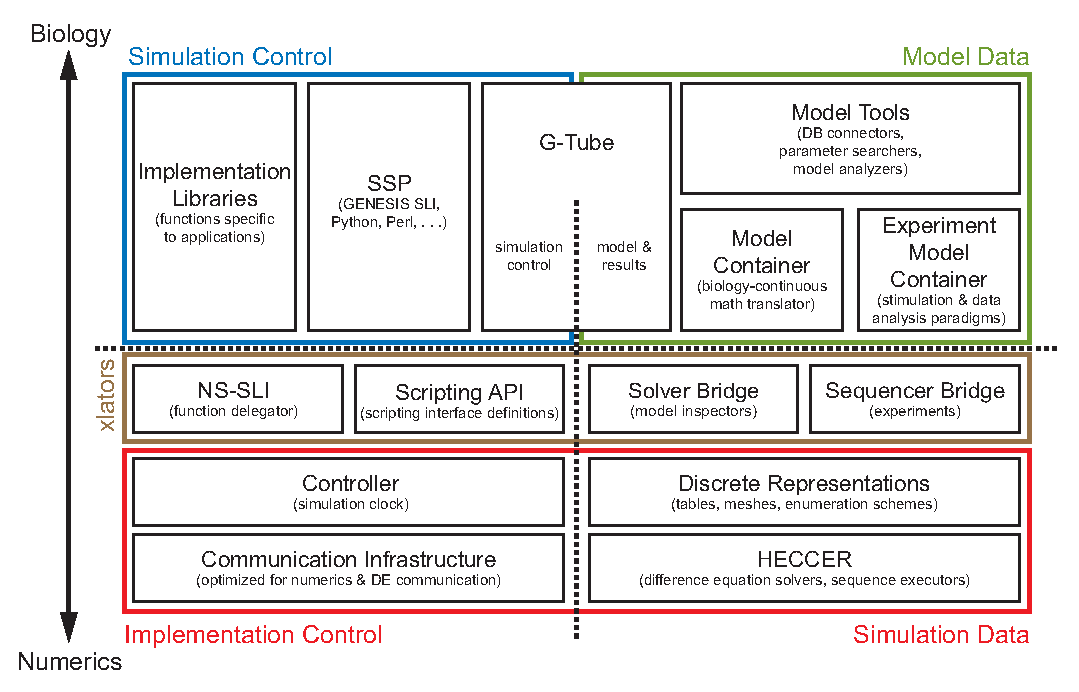
\includegraphics[width=4in]{figures/cbi-g3.eps}
%  \includegraphics[scale=0.4]{figures/cbi-level2.png}
\end{center}
\caption{
{\bf GENESIS 3.0.}
The first implementation of the Computational Biology Initiative federated software architecture.
}
\label{fig:cbi_g3.eps}
\end{figure}

\clearpage

% Figure 2
\begin{figure}[ht]
\begin{center}
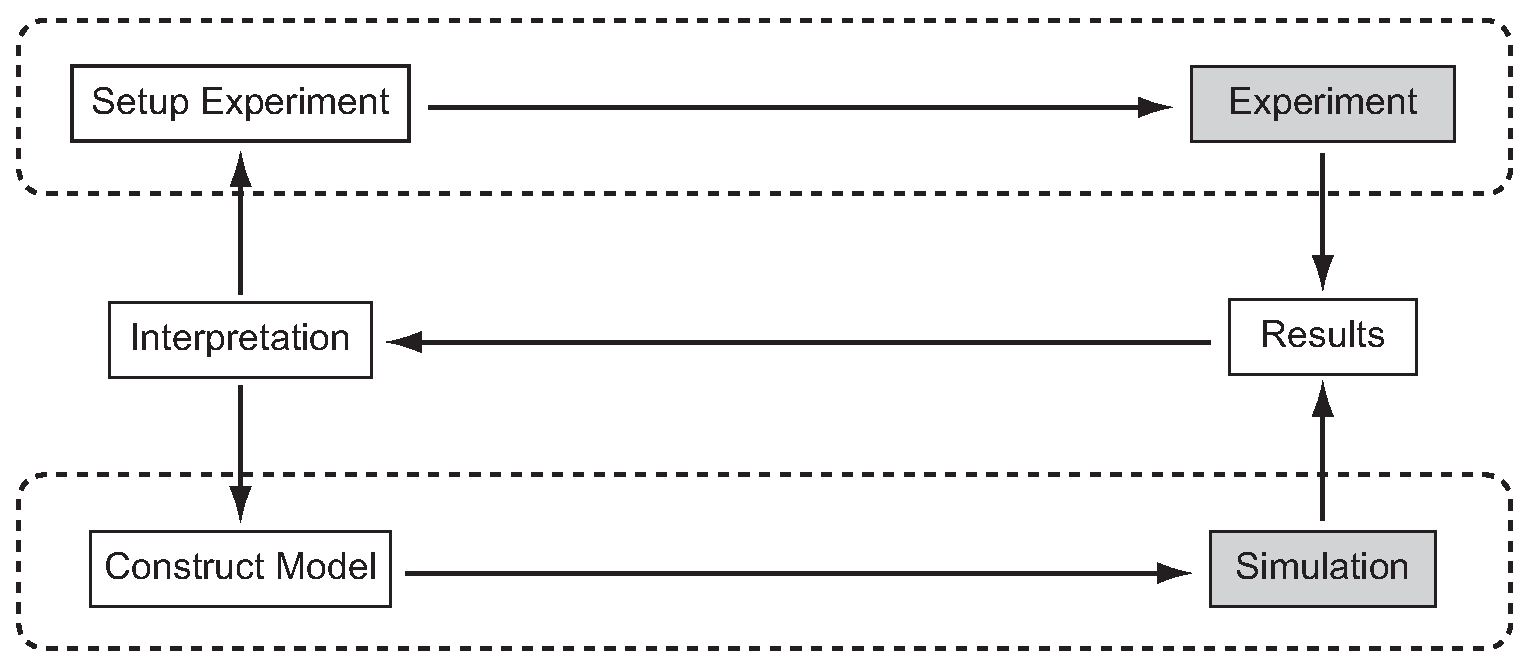
\includegraphics[width=4in]{figures/exp-sim.eps}
\end{center}
\caption{
{\bf Data flows in science.}
Conducting experiments and running simulations are two iterative processes indicated by the upper and lower dashed outlines. They are connected by an interposed feedback loop that uses the iterative interpretation of results to design new experimental setups and model constructions.
}
\label{fig:data-flows}
\end{figure}

\clearpage

% Figure 3
\begin{figure}[ht]
\begin{center}
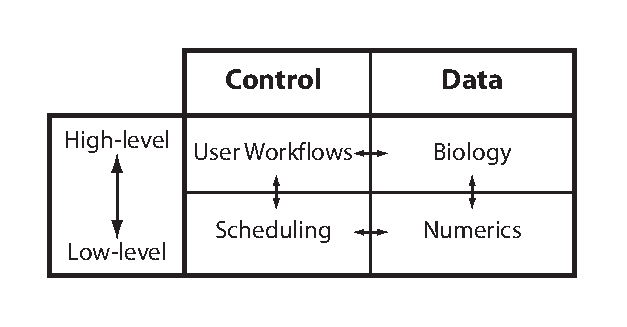
\includegraphics[width=4in]{figures/matrix.eps}
\end{center}
\caption{ {\bf Principle concerns.}  The four fundamental building
  blocks of a simulator are distinguished by separating (i) Data from
  control, and (ii) High level biological concepts from their
  mathematical implementation. In a federated architecture the only
  allowed interactions between modules are those indicated by the
  vertical and horizontal arrows. Diagonal interactions are forbidden
  as they ultimately lead to interactions that result in the creation
  of a monolithic software architecture.  }
\label{fig:data-control}
\end{figure}

\clearpage

% Figure 4
\begin{figure}[ht]
\begin{center}
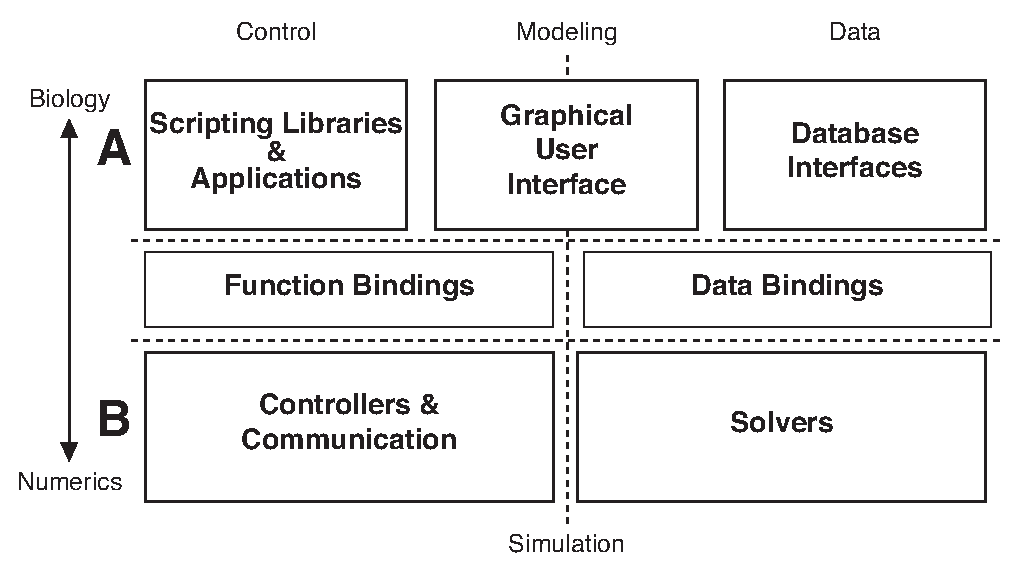
\includegraphics[width=4in]{figures/cbi-architecture-simple.eps}
\end{center}
\caption{
{\bf A federated software architecture.}
}
\label{fig:cbi-architecture-simple}
\end{figure}

\clearpage

% Figure 5
\begin{figure}[ht]
\begin{center}
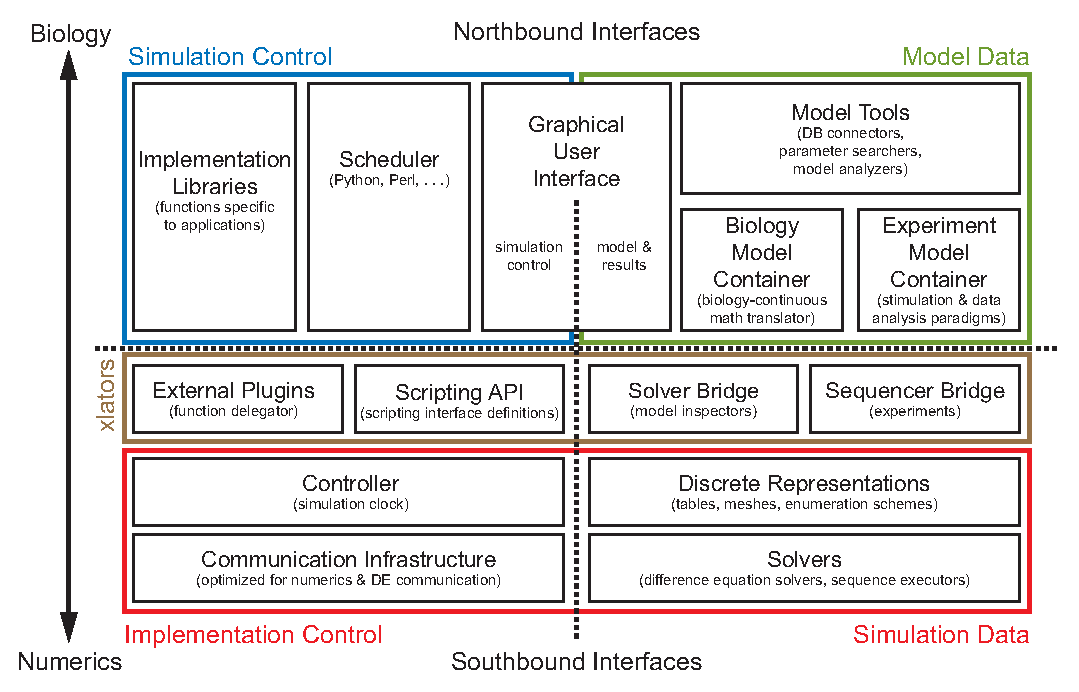
\includegraphics[width=4in]{figures/cbi-architecture-expanded.eps}
\end{center}
\caption{
{\bf The Computational Biology Initiative federated software architecture.}
}
\label{fig:cbi-architecture-expanded}
\end{figure}

\clearpage

%\section*{Tables}
%\begin{table}[!ht]
%\caption{
%\bf{Table title}}
%\begin{tabular}{|c|c|c|}
%table information
%\end{tabular}
%\begin{flushleft}Table caption
%\end{flushleft}
%\label{tab:label}
% \end{table}

\begin{table}[!ht]
\caption{
\bf{Table title}}
\begin{tabular}{|c|c|c|}
%table information
\end{tabular}
\begin{flushleft}
\end{flushleft}
%\label{tab:cbi-codecounts}
\end{table}

\end{document}
